%% AgenticAI4HPC'26 (SC26 workshop) — up to 10 pages, IEEE two-column, single-blind.
%% Compiles as-is on Overleaf (IEEEtran is built in). Draft: our results are real;
%% \todo{...} marks content still owed. Search "\todo" to find every open item.
\documentclass[conference]{IEEEtran}
\IEEEoverridecommandlockouts

\usepackage{cite}
\usepackage{amsmath,amssymb,amsfonts}
\usepackage{graphicx}
\usepackage{booktabs}
\usepackage{xcolor}
\usepackage{url}
\usepackage[hidelinks]{hyperref}
\usepackage{listings}

% --- draft-only helper: a visible TODO marker. Remove \usepackage before camera-ready. ---
\newcommand{\todo}[1]{\textcolor{red}{\textbf{[TODO: #1]}}}

\lstset{basicstyle=\ttfamily\footnotesize,columns=fullflexible,breaklines=true,
        frame=single,framesep=3pt,xleftmargin=3pt}

% --- Float placement: this paper is float-heavy (4 double-column figures + 5 tables).
% With LaTeX's stock parameters the floats cannot be packed onto text pages, so they
% cascade to the end and leave half-empty pages behind. These let more of the page be
% float and shrink the text LaTeX insists on keeping. Standard values; no extra package.
\renewcommand{\topfraction}{0.9}        % up to 90% of a page may be top floats
\renewcommand{\bottomfraction}{0.7}
\renewcommand{\textfraction}{0.07}      % as little as 7% text is acceptable
\renewcommand{\floatpagefraction}{0.75} % a float page must be 75% full (avoids near-empty pages)
\setcounter{topnumber}{3}
\setcounter{bottomnumber}{2}
\setcounter{totalnumber}{4}

\begin{document}

\title{Works but Wrong: Static Diagnosis of\\ HPC Simulation Setup Errors for AI Agents}

\author{
\IEEEauthorblockN{Youngsung Kim}
\IEEEauthorblockA{Oak Ridge National Laboratory\\
Oak Ridge, TN, USA}
\and
\IEEEauthorblockN{Sudershan Gangrade}
\IEEEauthorblockA{Oak Ridge National Laboratory\\
Oak Ridge, TN, USA}
\and
\IEEEauthorblockN{Mario Morales Hern\'{a}ndez}
\IEEEauthorblockA{I3A-Universidad de Zaragoza\\
Zaragoza, Spain}
}

\maketitle

% Disable IEEEtran's em-dash substitution for repeated author names (see references.bib).
\bstctlcite{IEEEtran:BSTcontrol}

\begin{abstract}
A scientific HPC run often ``works but is wrong'': the solver launches, runs for hours of
compute time, and returns output that looks normal but is silently incorrect. The cause is not a
crash but a fault in the run's \emph{setup files}---the configuration and input files the solver
reads. The solver itself does not flag such a fault: the solver either rejects the files with a
cryptic message, or runs on and silently corrupts the result. We ask whether a small,
purpose-built tool, given to an AI coding assistant, measurably improves the assistant's ability
to \emph{debug} such runs. We present \textbf{\texttt{diagnose\_project}}, a static diagnosis
tool for the TRITON flood-simulation solver, delivered through the Model Context Protocol (MCP)
and as an in-editor tool. The tool works from the setup files alone---reading exactly what the
solver reads---and returns ranked, evidence-backed findings; the tool never runs the solver, so
diagnosis is safe and fast. We evaluate the tool on a test set of 32 TRITON projects with
deliberately injected faults. The experiment compares the \emph{same} agent \emph{with} the tool
(the \emph{+tool} arm) and \emph{without} the tool (the \emph{bare} arm), run in isolation on two
AI clients: Claude (\texttt{claude-sonnet-5}) and Codex (\texttt{gpt-5.6-sol}). Without the tool,
an agent already \emph{finds} most faults ($91$--$96\%$), so the tool is not a rescue. Instead,
the tool has three sharper effects. First, the tool lifts detection to \textbf{100\%} and---more
tellingly---raises how often the agent points at the \emph{right} fault, not merely a real one,
from \textbf{$78$--$80\%$} to \textbf{$98\%$}. Second, the tool reduces false alarms on clean
projects for the weaker client: Claude's false alarms fall from $3/12$ to $1/12$, while Codex
already raises none. Third, the tool \emph{reduces} cost---\textbf{$\sim$1.3--1.6$\times$ fewer}
back-and-forth turns, \textbf{$\sim$2--4$\times$ fewer} output tokens, and $1.6$--$3.8\times$
less wall-clock time---at under \textbf{1.5\%} overhead. Finally, we validate the tool on a
\emph{real} operational project, where the tool statically catches---in about a second---an
out-of-range runoff-indexing bug that silently corrupted a production GPU run. We generalize
that one fix into a family of count-and-reference checks and add fixtures from the real case.
Along the way we find that test fixtures must be validated against the real solver: a subtle
mismatch in our fixtures broke no test, yet quietly inflated the tool's measured advantage until
we caught the mismatch by running every fixture through the solver.
\end{abstract}

\begin{IEEEkeywords}
agentic AI, HPC workflows, LLM tool use, Model Context Protocol, scientific software,
static analysis, human-in-the-loop
\end{IEEEkeywords}

\section{Introduction}
\label{sec:intro}

When a high-performance computing (HPC) simulation \emph{crashes}, the failure is at least
honest: the program stops, and the program usually says why. The more expensive failure is the one
that stays quiet---the run that \emph{works but is wrong}. The solver launches, holds an
expensive compute node for hours, and writes results that look normal but are silently
incorrect. The cause is usually not a bug in the solver. The cause is a mistake in what the
scientist handed to the solver: an input grid of the wrong size, a rainfall file that is accidentally
all zeros, a fill-in-the-blank template that was never filled in, or a stated file count that
does not match the files on disk. We call the bundle a solver reads---the plain-text
configuration file plus the input data that file points to---the run's \emph{setup files}.
Experienced users learn to catch these setup-level mistakes by eye, but only slowly. Teaching
that skill to an AI assistant is what this paper is about.

AI coding assistants---agents that read a project's files and run commands on the project's
behalf---are increasingly used to set up and run such
simulations~\cite{lara,matclaw,mada,materials-aurora,mlipilot}. So it is natural to ask an
assistant directly, ``is this project configured correctly?'' Without a tool built for the job,
the agent answers by improvising: the agent reads whatever material is available---documentation,
sample projects, the solver's own source---and reconstructs the file conventions from that
material. Prompting alone does not make this improvisation reliable. The reason is that the
conventions---how a binary grid's header is laid out, or how the solver indexes the tables it
reads---are often undocumented, or documented only in part. The solver's source code is then the
only authoritative reference, and the agent must re-derive the conventions from that code on
every project~\cite{matclaw}. Working this way, the agent can often tell that \emph{something} is
wrong, but not reliably \emph{which} thing: the agent misidentifies the exact
fault~\cite{swebench,sweagent}, and can flag sound projects as
broken~\cite{sast-llm-compare}. This paper asks a narrow, testable question: \emph{if we give the
agent one small, purpose-built tool that encodes those conventions and inspects the project for
the agent, does the agent's fault-finding measurably improve, and at what cost?} The tool we
build, \texttt{diagnose\_project}, does exactly that: the tool reads a TRITON project's
configuration file and input files and reports faults \emph{without ever running the solver}.

We study this question with TRITON~\cite{triton,tritondocs}, an open-source flood-simulation
solver developed at Oak Ridge National Laboratory. TRITON solves the full 2D shallow water
equations to model flood propagation across heterogeneous terrain, and is routinely used for
operational flood forecasting; TRITON can run on one or many GPUs. A
single TRITON run is described entirely by a plain-text \texttt{.cfg} configuration file together
with the input files that file names---mostly \emph{rasters} (grids of values covering the
terrain, such as ground elevation) and time series---runoff hydrographs, tabulating discharge
per zone. These files are
exactly where the setup-level mistakes we study live. Our tool, \texttt{diagnose\_project},
inspects these files, and has three defining properties:
\begin{itemize}
  \item \textbf{It works from the project's own files.} It reads the solver's own \texttt{.cfg}
        configuration file and the input files it names, so it works on \emph{any} TRITON
        project---even one a person assembled by hand, not only the ones our own interface produced.
        In other words, it reads \emph{exactly what the solver reads}: the setup files the solver
        actually loads are its single source of truth.
  \item \textbf{It never runs the solver.} Every check is computed from those setup files alone.
        This makes diagnosis fast, and safe to run at any time---\emph{before} a run,
        to avoid wasting compute, and \emph{after} one, to explain a result the solver quietly got
        wrong. Because it inspects without executing, we call it a \emph{static} check.
  \item \textbf{One implementation, offered wherever the agent lives.} The same core logic is
        offered to agents two ways: as a Model Context Protocol (MCP) server for external agents such as
        Claude Code or Codex, and as a built-in tool inside the VS~Code Copilot editor. Any action that would change files
        first asks the user for approval.
\end{itemize}

Static diagnosis suits this setting because a TRITON run is declared rather than assembled: the
\texttt{.cfg} names its files and parameters, and each input is a self-contained raster or table.
The faults are correspondingly declarative---counts that disagree with the files, zone ids past a
declared range, headers that violate what the solver assumes---rather than emergent runtime state.

Finding the fault is only the first step of \emph{debugging} a broken run; the full loop is to
detect, understand, fix, and verify. We package \texttt{diagnose\_project} inside the open-source
Triforge Visual Studio Code Extension~\cite{triforge} (``the Triforge extension'' below), which
supports this whole loop, and
Section~\ref{sec:realworld} walks through the loop end-to-end on a real operational bug. This
paper measures only the first step---detection---in a controlled way; the later steps appear in
that case study as a demonstration rather than as separately measured claims.

\noindent\textbf{Contributions.}
\begin{enumerate}
  \item A static diagnosis tool for a real HPC solver that works from exactly the files the solver
        reads, built so that a single piece of pure logic drives every surface and never launches a
        process, and delivered to agents in two forms (Section~\ref{sec:design}).
  \item A test set of 32 TRITON projects with known, labeled faults, and a controlled experiment
        that compares the \emph{same} agent with and without the tool---a ``$\pm$tool
        ablation''---across two independent AI clients, each run in its own isolated sandbox
        (Section~\ref{sec:method}).
  \item A transparent, end-to-end evaluation, published for inspection. A $\pm$tool ablation
        isolates \emph{where} the tool helps---sharper fault localization, fewer false alarms, and
        lower cost, not better raw detection---and a real operational run validates the tool end-to-end on
        a bug that had silently corrupted a production GPU job (Section~\ref{sec:realworld},
        Figure~\ref{fig:beforeafter}). Every per-fixture verdict, transcript, and ground-truth label
        is browsable online as reviewer
        artifacts~\cite{artifact-tool,artifact-oracle,artifact-ablation,artifact-human}.
\end{enumerate}

The diagnosis tool is one instance of a broader idea we call \emph{agent-legible HPC}
(Section~\ref{sec:pattern}): designing scientific workflows so that an AI agent can inspect and
act on them safely. In this paper we evaluate only the diagnosis instance. We begin with the real
failure that prompted the tool.

\section{Motivating Example}
\label{sec:motivation}

\begin{figure*}[!t]
\centering
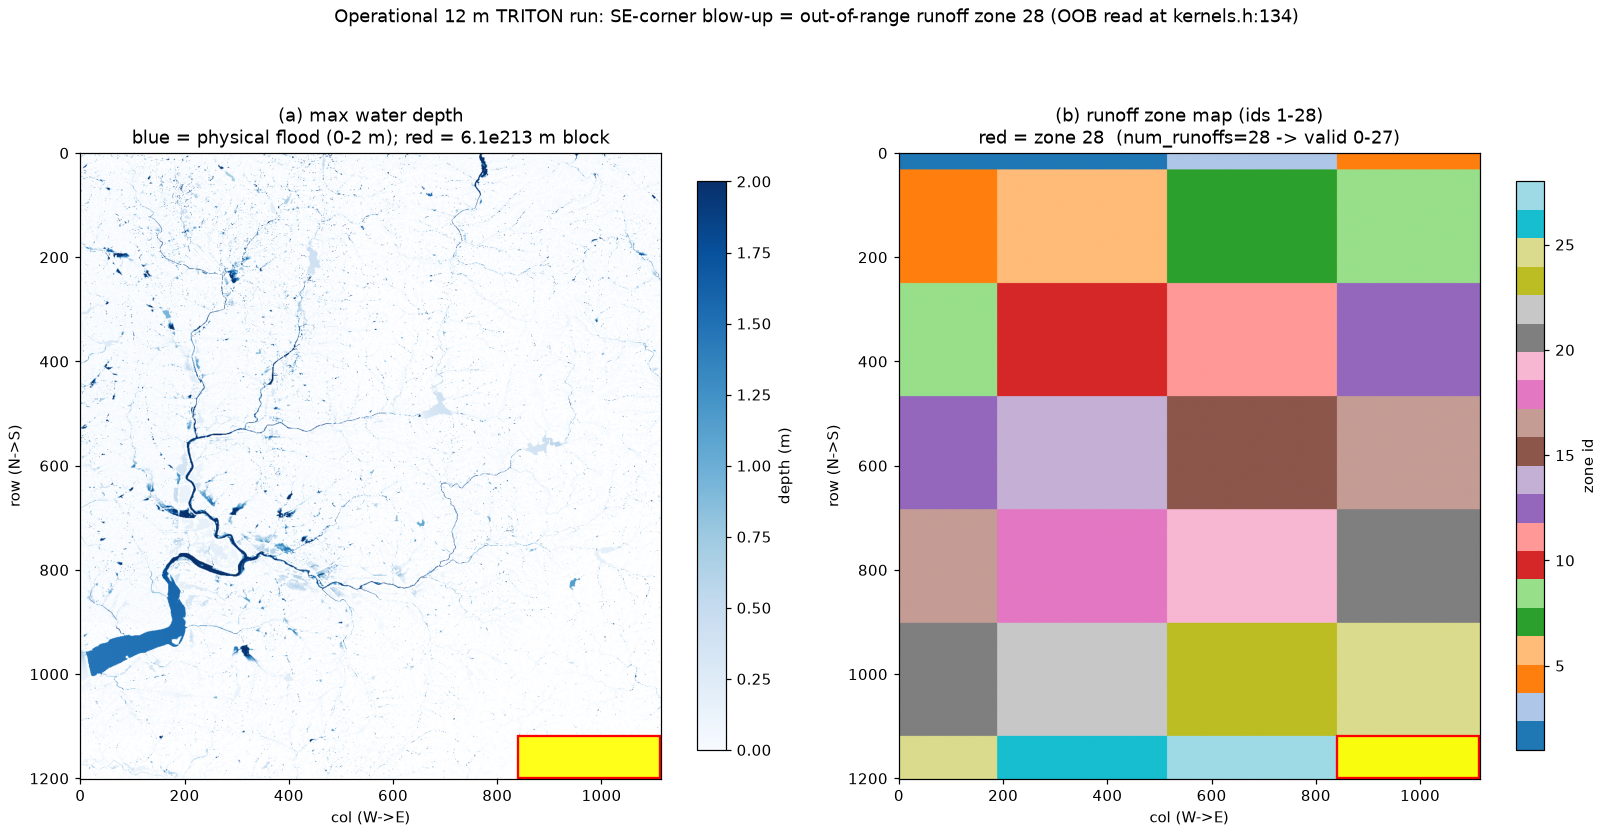
\includegraphics[width=0.60\textwidth]{figures/operational-anomaly.png}
\caption{A real ``works-but-wrong'' failure in an operational TRITON run
($4458\times4802$ cells at 12\,m). (a)~Final maximum water depth: a physical dendritic flood
(blue, $0$--$2$\,m) \emph{plus} a hard-edged $6\times10^{213}$\,m block in the southeast
(red). (b)~The runoff zone map: the block sits exactly on zone~28. With
\texttt{num\_runoffs}=28 and 0-based indexing, that reads one entry past the runoff table.
Nothing crashed; the tool flags this from the setup files alone.}
\label{fig:anomaly}
\end{figure*}

Figure~\ref{fig:anomaly} comes from a real, operational TRITON flood forecast---a daily forecast
produced by a system still under active development. The solver ran
on GPUs, finished in about $27$~minutes, and wrote a complete set of output maps, reporting success. Yet
the map of maximum water depth (panel~a) contains a sharp-edged rectangular block of water in
the domain's southeast corner holding a physically impossible $6\times10^{213}$\,m, while the
rest of the map is a believable branching flood (at most $21$\,m). A domain expert could see
at a glance that the block was wrong. Finding out \emph{why} was far harder: even domain
scientists could not point to the root cause without cross-checking the configuration file, the
contents of the input data files, and finally the solver's source code.

The cause is an off-by-one indexing error---the kind no crash ever reveals. TRITON adds rainfall
runoff using two inputs: a \texttt{runoff\_map} that tags every grid cell with a zone number, and
one runoff hydrograph per zone. To apply the rain, the solver takes a cell's zone number
and uses it directly to index the table of series. It never checks that the number is in range.
That check mattered here. The upstream pipeline---not the solver---numbered the zones from $1$ to
$28$, but the solver fills its table from $0$, so its valid slots run only $0$ to $27$. Zone $28$
therefore fell one slot past the end. The solver read whatever sat in the next piece of memory and
poured that raw bit pattern, read back as a float, into every cell of the zone. Because the zones
run northwest to southeast,
that zone is the block in the far southeast corner (panel~b)---a clean rectangle exactly where the
numbering went past the end of the table.

This is the ``works but is wrong'' failure in its purest form. A setup-level mistake---a map
numbered from $1$ feeding a table indexed from $0$---never shows up in the run's success/failure
status, yet the mistake wastes the run and can corrupt a flood-forecast product. A \emph{static}
check can catch this mistake: the largest zone number in the map and the declared number of
zones both sit in the setup files, so no solver run is needed to notice that the two disagree.
Section~\ref{sec:realworld} returns to this bug to show the tool catching it---and the fix.

\section{\texttt{diagnose\_project}: Design}
\label{sec:design}

\texttt{diagnose\_project} reads a TRITON project's setup files---the configuration file and the
inputs that file points to---and reports the faults it finds, without ever running the solver.
The tool follows one design principle: a single, self-contained core of logic that the agent
calls directly. The core is a pure function of the parsed setup files, with no dependence on any
editor or operating-system feature. The same code therefore runs three ways---inside an editor,
inside an automated test job, or through an external agent such as Claude Code or Codex
(Figure~\ref{fig:architecture}). This design is one instance of a broader pattern we call
\emph{agent-legible HPC}, which Section~\ref{sec:pattern} describes.

\begin{figure*}[!t]
\centering
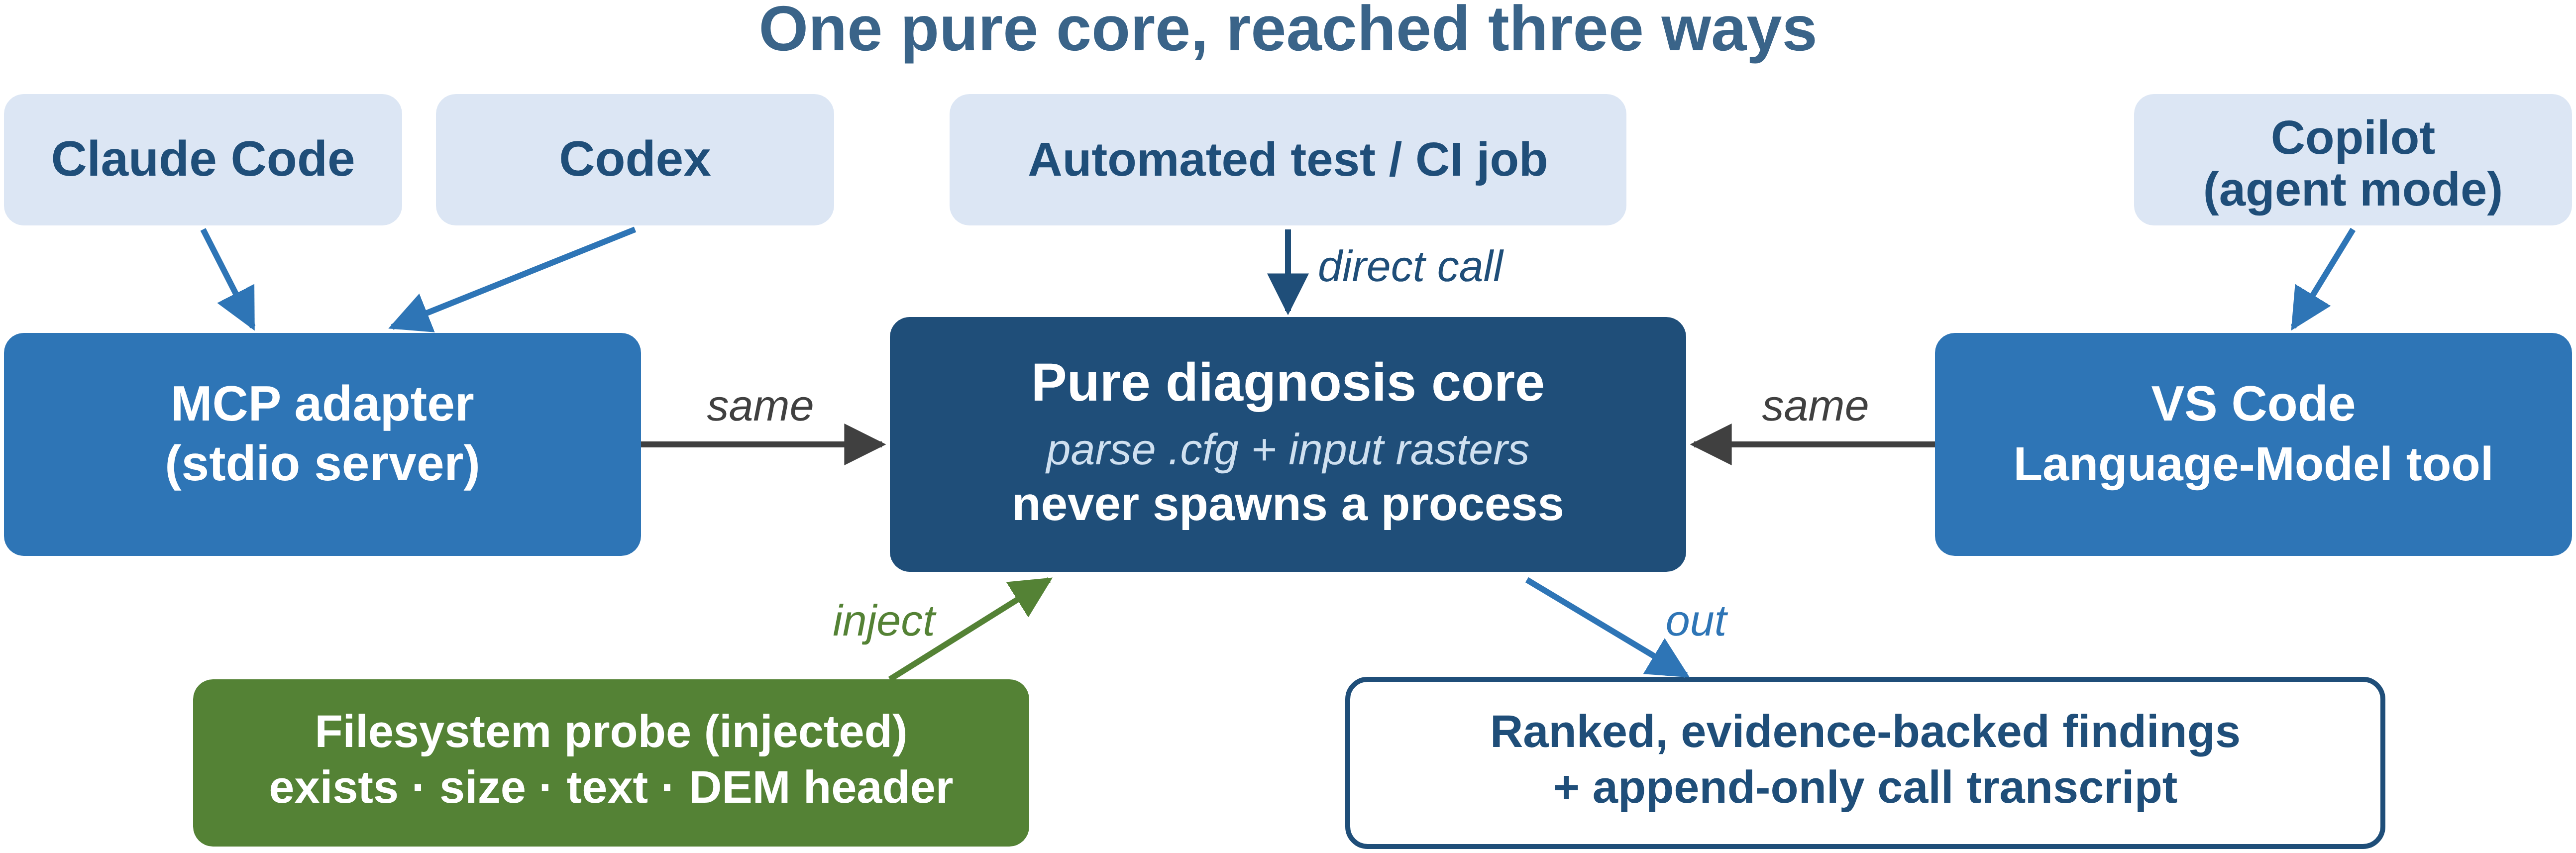
\includegraphics[width=\textwidth]{figures/architecture.png}
\caption{One shared core, reached three ways. The core parses the
\texttt{.cfg} and its input grids through a file-access helper supplied from outside, and never
launches a process or imports editor or operating-system code. External agents such as Claude
Code or Codex reach it through the MCP wrapper, the in-editor Copilot through the VS~Code
wrapper, and an automated test or CI job calls it directly. It returns ranked, evidence-backed
findings plus an append-only log of every call.}
\label{fig:architecture}
\end{figure*}

\subsection{What it checks}
The tool reads the TRITON \texttt{.cfg} configuration file---a simple list of \texttt{key=value}
settings---and the input files that file points to, and returns a ranked list of \emph{findings}. Each
finding carries a severity, a short plain-language explanation of the evidence, and a pointer to the
file or step to look at. Table~\ref{tab:checks} lists the full set of checks. Every check is static:
computed from the setup files, with no solver run.

\begin{table}[!t]
\caption{Static check catalog. Every check works from the setup files the solver reads and requires
no solver run; together they test the setup against the conventions the solver silently assumes.}
\label{tab:checks}
\centering
\footnotesize
\resizebox{\ifdim\width>\columnwidth\columnwidth\else\width\fi}{!}{%
\begin{tabular}{@{}ll@{}}
\toprule
\textbf{Check} & \textbf{Fault it catches} \\
\midrule
unsubstituted-placeholder & template token left in the config (e.g.\ \texttt{XX..XX}) \\
missing-input-file        & a referenced input file is absent \\
degenerate-forcing        & the active forcing series is all zeros \\
grid-size-mismatch        & an input raster's grid $\neq$ the DEM grid \\
hydrograph-coverage       & forcing ends before \texttt{sim\_duration} \\
value-range-sanity        & out-of-range parameter (e.g.\ Courant, Manning) \\
unsupported-input-format  & \texttt{input\_format} not \texttt{BIN}/\texttt{ASC} (e.g.\ \texttt{GTIFF}) \\
bin-raster-header\textsuperscript{\S}     & a \texttt{.bin} raster's header wrong for its role \\
hydrograph-delimiter\textsuperscript{\S}  & a forcing row is whitespace- not comma-delimited \\
\midrule
\multicolumn{2}{@{}l@{}}{\emph{count-and-reference integrity} family:} \\
\quad runoff-column-mismatch    & \texttt{num\_runoffs} $\neq$ runoff hydrograph columns \\
\quad source-count-mismatch     & \texttt{num\_sources} $\neq$ source rows/columns \\
\quad runoff-map-zone-range$^\dagger$ & a \texttt{runoff\_map} zone id $\geq$ \texttt{num\_runoffs} \\
\quad extbc-count-mismatch$^\dagger$  & \texttt{num\_extbc} $\neq$ external-boundary entries \\
\midrule
\multicolumn{2}{@{}l@{}}{\emph{physical-plausibility layer} (advisory; warn, never block):} \\
\multicolumn{2}{@{}l@{}}{\quad frictionless domain (Manning $n{=}0$, unbounded velocity), Manning/Courant out of range,} \\
\multicolumn{2}{@{}l@{}}{\quad non-positive \texttt{h\_extra}, negative runoff, no raster output, deep DEM pits} \\
\midrule
\multicolumn{2}{@{}l@{}}{\emph{user-rule layer} (user-declared invariants, verified):} \\
\multicolumn{2}{@{}l@{}}{\quad inputs present, \texttt{numRunoffs}, \texttt{numSources}, \texttt{simDurationSec}, forcing range} \\
\bottomrule
\end{tabular}}

\smallskip
{\footnotesize $^\dagger$ Added from the real-world case of Section~\ref{sec:realworld};
each maps to a specific unchecked read in the solver, and the zone-range check is the one that
catches a 1-based map feeding a 0-based table. \textsuperscript{\S}~Surfaced by the solver-oracle
validation of Section~\ref{sec:oracle}: running fixtures against the real build exposed two
binary/text format invariants the solver silently requires. Validated at the tool level and,
for $^\dagger$, on the real project; the $\pm$tool ablation of Section~\ref{sec:results} was run
on the upgraded tool and so exercises all four.}
\end{table}

\subsection{How it is built: one core, thin wrappers, no launching}
The diagnosis logic is written as a \emph{pure} function: given the parsed configuration and a
small file-access helper, the function always returns the same findings and changes nothing on
disk. The helper reports whether a file exists, its size, its text, and---after the fidelity fix
of Section~\ref{sec:method}---the header of a binary elevation grid. The helper is supplied from
the outside, so the core itself imports no editor or operating-system code and never launches
another program. Each delivery form plugs in its own real file-access helper. The payoff is that
a single body of logic can be tested entirely in memory, run without a graphical interface, and
behave identically whether the logic is reached over MCP or from inside the editor.

\subsection{Three ways to reach the same tool}
The same core is reached three ways---two put it in front of an agent, and the third calls it directly:
\begin{itemize}
  \item \textbf{As an MCP server}~\cite{mcp}: external agents (Claude Code, Codex, Claude Desktop)
        start a small server process and call the tool over MCP.
  \item \textbf{As a built-in editor tool}: VS~Code Copilot, acting on the user's behalf, calls the
        same core directly. The
        ranked findings return as text into the Copilot chat (the user can also invoke the tool
        explicitly as \texttt{\#diagnoseProject}).
  \item \textbf{As a direct call to the core}: a script, batch job, or automated test calls the pure
        diagnosis function directly---no server, no editor, no agent in between. This is the generic,
        raw path: the same core the two surfaces above wrap, and the way the test suite exercises it.
\end{itemize}

\texttt{diagnose\_project} is one of nine tools the extension offers (Table~\ref{tab:tools}), and
returns the same findings whichever way the tool is reached.

\begin{table}[!t]
\caption{The Triforge extension's agent tool set, exposed identically on the MCP and in-editor
surfaces. \texttt{diagnose\_project} (this paper's focus) and \texttt{explain\_triton} are
read-only; $^\ddagger$ marks state-changing tools gated behind an approval handshake; the rest
write project-local files without a gate.}
\label{tab:tools}
\centering
\footnotesize
\resizebox{\ifdim\width>\columnwidth\columnwidth\else\width\fi}{!}{%
\begin{tabular}{@{}ll@{}}
\toprule
\textbf{Tool} & \textbf{Purpose} \\
\midrule
diagnose\_project            & static fault diagnosis from the solver's own files (read-only) \\
explain\_triton              & curated TRITON/extension knowledge base (read-only) \\
configure\_solver            & render/update the \texttt{.cfg} configuration file \\
export\_tfp                  & bundle a project into a portable \texttt{.tfp} \\
animate\_gif                 & render an output variable to a GIF \\
run\_local$^\ddagger$        & run a build/solver command locally \\
import\_tfp$^\ddagger$       & unpack a \texttt{.tfp} into a project \\
create\_water\_source$^\ddagger$ & add streamflow sources + hydrographs \\
generate\_dem$^\ddagger$     & fetch/build a DEM for the domain \\
\bottomrule
\end{tabular}}
\end{table}

\section{The Agent-Legible HPC Pattern}
\label{sec:pattern}

All of the Triforge extension's tools, including \texttt{diagnose\_project}, are built the same way: a self-contained
core an agent can call directly (Table~\ref{tab:tools}). Our
goal across all these tools is \emph{agent-legible HPC}: exposing an HPC workflow---its setup
files, conventions, and state---in a form an agent can read and understand, so that the agent can
inspect the workflow and act on it safely.

The Triforge extension reaches this legibility through four patterns that wrap the tools, each addressing one part
of that goal. The first makes the workflow \textbf{readable}: each project ships small plain-text
files, \texttt{AGENTS.md} and \texttt{CLAUDE.md}, that say what the project is and how it is laid out,
so an agent understands the project just by reading these files. The second keeps action \textbf{safe}: a read-only
tool such as diagnosis runs on its own, but any tool that writes files or starts a run first stops and
asks the person to approve it, so an agent cannot quietly change a project or launch an expensive job
without consent. The third keeps a project \textbf{portable}: the commands \texttt{export\_tfp} and
\texttt{import\_tfp} bundle an entire project---its configuration, inputs, and outputs---into one file
that can move between a laptop and an HPC cluster; this is the path that later carried the corrected
run of Section~\ref{sec:realworld} back from the cluster to be re-checked. The fourth keeps action
\textbf{accountable}: every tool call is written to an append-only log, leaving a complete record of
what the agent did.

This paper measures only the diagnosis core, not the four patterns around it.

\section{Evaluation Methodology}
\label{sec:method}

\subsection{The test set of faulty and clean projects}
Our test set is \textbf{32} complete, self-contained TRITON projects
(\texttt{eval/diagnose-corpus/}): \textbf{15} that each contain one known defect, \textbf{5}
\emph{user-rule} projects---whose ``fault'' is that the setup files break a rule the user explicitly
declared---and \textbf{12} that are
deliberately clean (so we can check the tool does not raise false alarms). Together, the faulty
projects cover the range of things that go wrong: an input grid of the wrong size (in three
different file forms), the runoff-zone counting and out-of-range bugs of
Section~\ref{sec:realworld} (in both their silent and crashing versions), miscounted water sources
and boundaries, a landscape with zero friction everywhere, a rainfall file with the wrong
separator that the solver rejects, an unfilled template placeholder, a missing input file, and
out-of-range parameter values. They span both binary (\texttt{BIN}, $24$ projects) and text
(\texttt{ASC}, $8$ projects) input formats, and together they exercise every major input type:
terrain, rainfall runoff, water sources, friction, and starting water levels. A companion file
records the correct answer for every project---its format, its single injected fault (or
\texttt{clean}), and any user-declared rules. Each faulty project carries \emph{exactly one}
intended fault, so ``the right answer'' is unambiguous and naming a different problem counts as a
miss. The tool-level accuracy of Section~\ref{sec:results} and the with-versus-without comparison
both use all \textbf{32} projects. We generated the projects with AI assistance; the credibility
of the labels does not rest on that origin, because Section~\ref{sec:oracle} confirms every label
against the real TRITON solver.

\subsection{A subtle test-data bug we had to fix}
\label{sec:fidelity}
Making the test projects \emph{faithful} to the real solver turned out to matter to the result.
Our binary elevation grids were at first stored without a header. The real solver, however,
expects a six-number header (grid width and height, corner coordinates, cell size, and a no-data
marker) at the start of a binary elevation file and reads the data after that header; the other
binary inputs have no header (we confirmed all of this in the TRITON source). Those
header-less---and often all-zero---placeholder elevation files handed the tool-less agent a
believable but wrong complaint (``the binary inputs are missing their headers''). That wrong
complaint pushed aside the intended fault on the binary projects, and so \emph{overstated} the
tool's advantage. We rebuilt every binary project with a proper header and real terrain, taught
the tool to read the grid from that header exactly as the solver does, and re-ran everything.
Section~\ref{sec:results} reports the corrected numbers, and Section~\ref{sec:threats} draws the
lesson.

\subsection{The comparison: with the tool versus without, on two AI clients}
Our experiment compares two \emph{arms}---conditions that are identical except for one thing,
whether the tool is available:
\begin{itemize}
  \item \textbf{\emph{+tool}} (the treatment arm): the agent---the AI client---\emph{with}
        \texttt{diagnose\_project} available to call.
  \item \textbf{\emph{bare}} (the control arm): the \emph{same} agent, model, and instructions, but
        \emph{without} the tool---an ordinary language model that can still read files and run shell
        commands.
\end{itemize}
We name the two arms by what sets them apart (\emph{+tool} vs.\ \emph{bare}). We run each arm on two separate AI command-line clients---\textbf{Claude}
(\texttt{claude -p}, running the \texttt{claude-sonnet-5} model) and \textbf{Codex}
(\texttt{codex exec}, running \texttt{gpt-5.6-sol})---starting a brand-new session for each test. Both arms get the same neutral instruction: review the project and report any fault. The
\emph{+tool} arm gets one extra line noting that the tool is available.

\paragraph{Keeping each test isolated} A command-line agent can open files by absolute path, and
the test machine holds TRITON material in many places (the whole test set, the tool's own source
code, other projects). Setting a working directory alone is not enough to stop the agent from
reading those files. So each test runs inside a lightweight sandbox (\texttt{bwrap}) that hides
the real home directory and exposes only what the test needs: the language-model toolchain, the
client's login credentials, and the \emph{one} project under test. The agent can therefore see
only that project's \texttt{run.cfg} and its \texttt{input/} folder. For the \emph{+tool} arm, a
copy of the MCP server is placed where the agent can reach it, outside the hidden files.

\subsection{Scoring the answers, and keeping the comparison fair}
\label{sec:scoring}
The unit we score is a \emph{cell}: one fresh agent session on one project. To average out the
randomness in an agent's answers, we run each faulty project \textbf{three} times, and each clean
or user-rule project once. We report four numbers. \emph{found\%}: did the agent name the true
fault (or, for a clean project, correctly report no fault)? \emph{stage\%}: on a faulty project,
did the agent point at the \emph{right} file or step? This measure separates a genuine diagnosis
from ``right symptom, wrong cause,'' which a plain yes/no detection score would miss.
\emph{clean-precision}: \emph{found\%} on the clean projects only---in other words, how well the
agent avoids false alarms (``crying wolf''). \emph{cost}: the number of back-and-forth turns, the
wall-clock time, the tokens used, and the tool's own communication overhead
(Table~\ref{tab:efficiency}). The cost numbers answer the worry that calling the tool costs more
than it saves.

\begin{figure*}[!t]
\centering
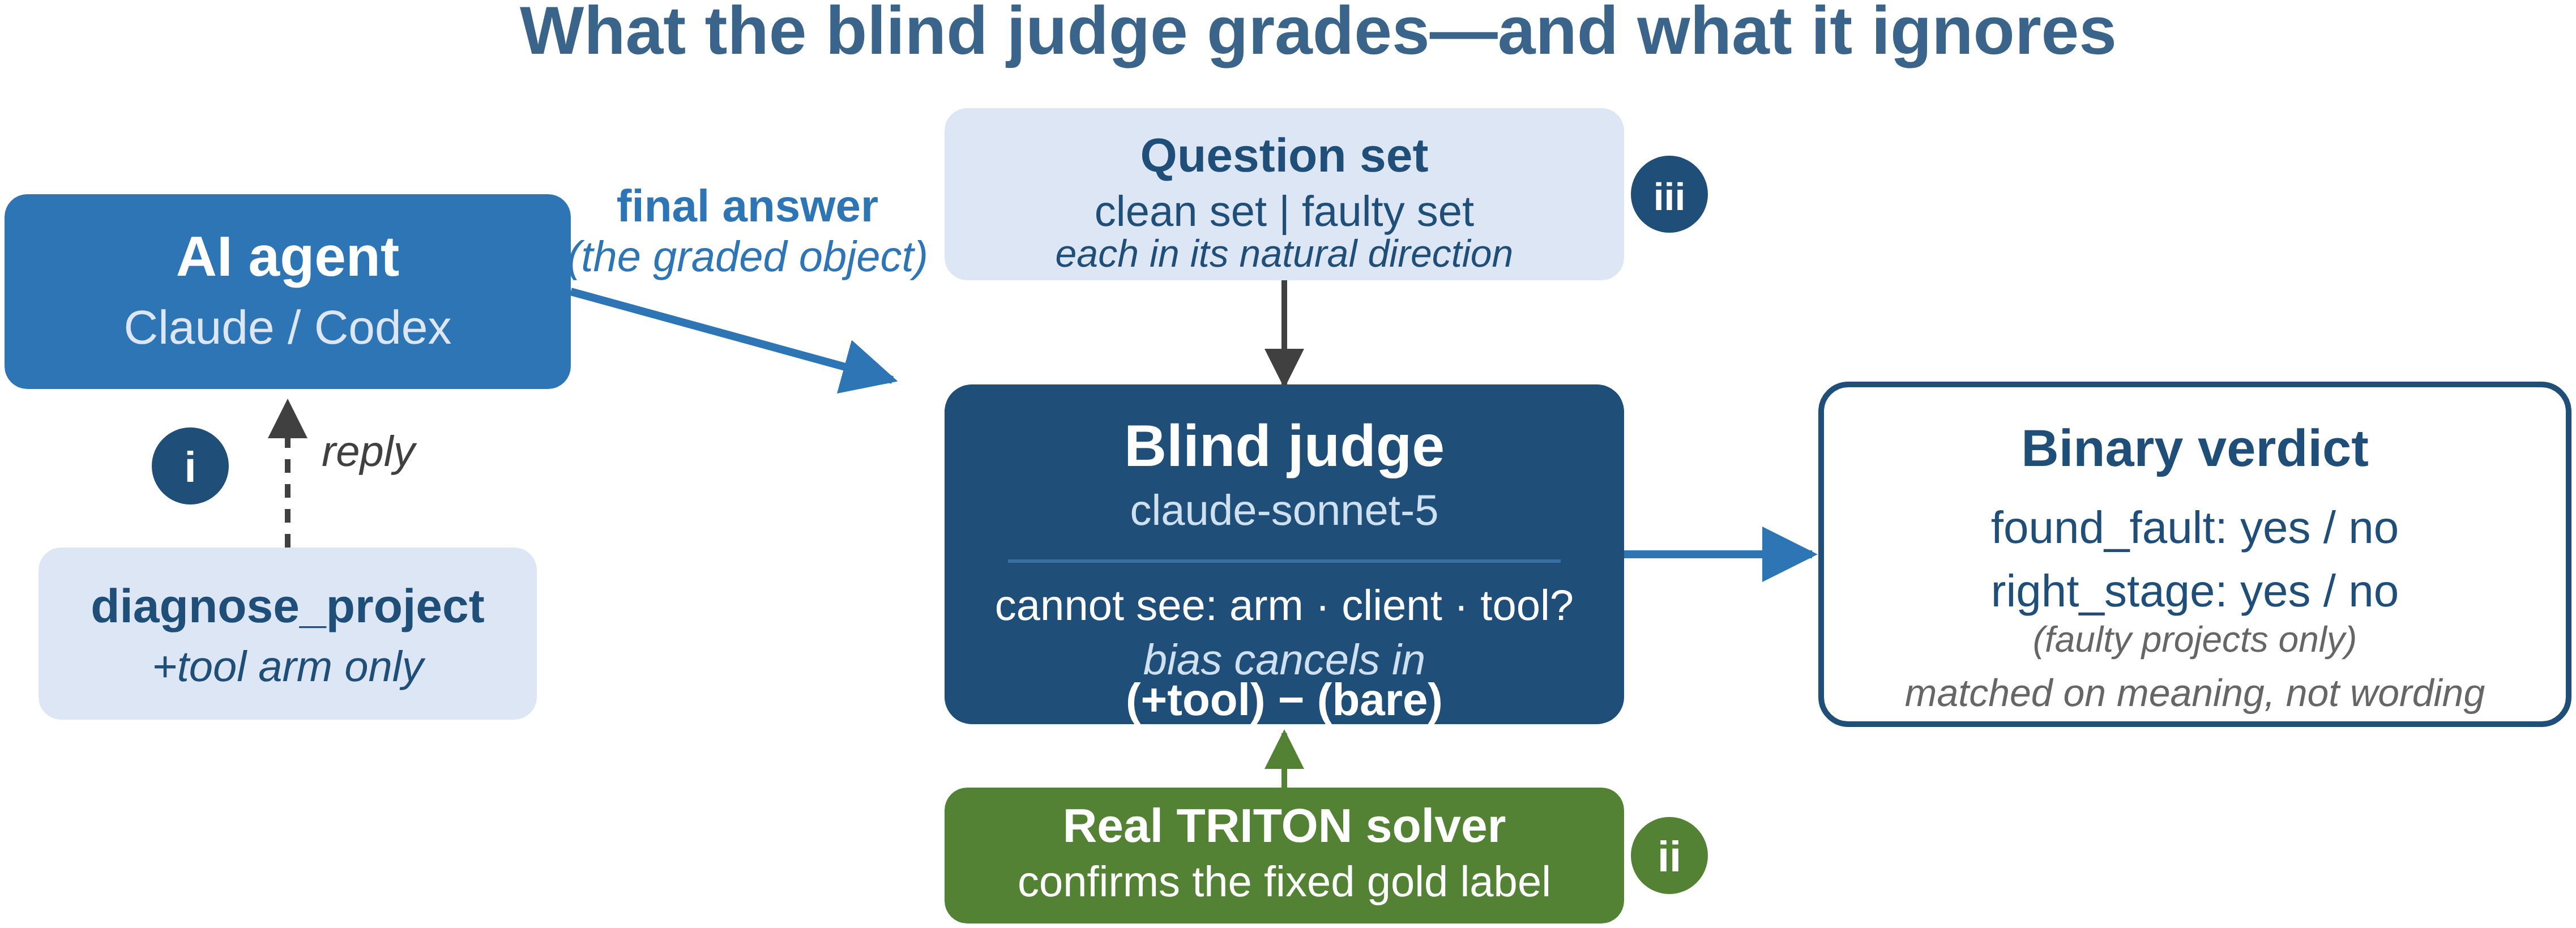
\includegraphics[width=\textwidth]{figures/fairness.png}
\caption{What the blind judge grades, and what it ignores. It scores only the agent's
\emph{final answer}, never \texttt{diagnose\_project}'s reply, which merely feeds the agent
(\textbf{i}); it grades against a \emph{fixed gold label} confirmed by the real TRITON solver,
not its own opinion (\textbf{ii}); and it asks clean and faulty projects separate,
natural-direction questions to avoid a double negative (\textbf{iii}). Blind to arm, client, and
tool, its bias cancels in the \mbox{\emph{+tool}\,$-$\,\emph{bare}} difference. The verdict is
binary and matched on meaning, not wording.}
\label{fig:fairness}
\end{figure*}

\paragraph{Why the comparison is fair} We grade every answer with a second language model
(\texttt{claude-sonnet-5}) acting as a \emph{blind judge} (Figure~\ref{fig:fairness}). The judge
sees \emph{only} the agent's answer and the project's known correct label. The judge never sees
which arm produced the answer, which client ran the session, or whether a tool was involved. This
blindness is the key control. Because the judge cannot tell the \emph{+tool} answers from the
\emph{bare} ones, any consistent bias applies \emph{equally} to both arms and \emph{cancels out}
in the \emph{+tool}-minus-\emph{bare} difference we report. What remains is the judge's plain
error rate, which we measure separately (Section~\ref{sec:threats}). Three further choices, shown
in Figure~\ref{fig:fairness}, guard against subtler leaks. (i)~The judge grades the agent's
\emph{own answer}, not the tool's reply, because the agent's answer is the only output both arms
produce; so if the tool gives a correct reply and the agent ignores that reply, the run still
scores as wrong. (ii)~The judge grades against a \emph{fixed} answer confirmed by the real solver
(Section~\ref{sec:oracle}), not against the judge's own opinion, so a mislabeled project cannot
corrupt the scores. (iii)~The judge asks clean projects and faulty projects separate questions,
each phrased in its natural direction; this removes a double-negative that had once mis-scored
valid projects. The verdict is a compact \emph{binary} label---\texttt{found\_fault} and, on
faulty projects, \texttt{right\_stage}---matched on meaning, not wording, and saved with a
one-line reason for human audit (Section~\ref{sec:threats}).

\section{Results}
\label{sec:results}

We report the results in two parts. The first part asks how accurate the tool is on its own. That
number only means something if the answer key we grade the tool against is correct, so we check
the key too---and neither check uses any AI. The second part asks the central question: does
handing the tool to an AI agent change what the agent finds?

\subsection{Tool-level accuracy, checked against the real solver}
\label{sec:oracle}
Run on its own against all \textbf{32} test projects, the tool gets every case right: the tool
flags every faulty project (\textbf{100\% detection}), makes the real fault its top finding with
nothing else competing (\textbf{100\% isolation}), and raises no false alarm on any clean project
(\textbf{100\% clean precision}). Re-running the shipped evaluation script reproduces these
numbers exactly (the script writes them to \texttt{report.json}). But a perfect score only shows
that the tool agrees with \emph{our own} answer key. A perfect score does not show that the key
itself is right, and a skeptic could fairly suspect that we built the test set to suit the tool.
To show that the key is right, we check the key against the program the key describes: we run
every project through the real TRITON build (\texttt{eval/diagnose-corpus/build}) and watch what
the solver does. Section~\ref{sec:realworld} adds a second, independent check---the tool on a
real project we did not build.

The solver can do one of three things: stop while loading the setup files, run to the end, or
start computing and then fail. Stopping or failing is a clear verdict: the project really is
broken. That verdict alone settles the \textbf{11} projects the solver refuses or kills; the tool
had flagged all \textbf{11}, so no broken project slips past the tool (Table~\ref{tab:oracle}).
Finishing, though, does not prove a project is correct: a run can finish and still write wrong
numbers, and that is the exact failure this tool is built to catch. So we never call a project
clean just because the solver finished. Each finished run also goes through an automatic check of
its output for obvious signs of trouble---values that are not real numbers, values far outside
any physical range, or output that is all zeros or a single repeated number. This automatic check
clears the clearly sound runs and flags the doubtful ones (Section~\ref{sec:reproducibility}).

Together the solver and this output check settle \textbf{22} of the \textbf{32} projects with no
human effort: the \textbf{11} the solver rejects, and \textbf{11} more that finish with clearly
sound output. The other \textbf{10} still need a person to judge (Table~\ref{tab:oracle}). Two of
the ten are the runs the output check flagged as doubtful. The remaining eight finish without
complaint yet are still faults a user would want caught: most break a rule the operator stated or
use a physically implausible setting, and one, \texttt{fault-runoff-zone-oob}, finishes with
output that looks fine but is silently wrong. That last case shows best why finishing is not
enough. The project contains the same out-of-range read as in Section~\ref{sec:motivation}, but
on a small grid; instead of crashing (as the read does on the large grid), the bad read lands on
harmless memory, and the run ends with quietly corrupted results---and the tool flags the project
anyway. So the real solver does not remove the need for human judgment; the solver shrinks that
need, from all \textbf{32} project labels to about \textbf{10}.

\begin{table}[!t]
\caption{The \textbf{32} test projects, grouped by how each label was settled. The solver decides
\textbf{22} cases on its own---\textbf{11} it rejects or crashes on, \textbf{11} it finishes with
sound output. The other \textbf{10} need a person: \textbf{2} the output check flags as doubtful,
and \textbf{8} that finish normally yet are faulty. The tool independently flags all \textbf{11}
broken and all \textbf{8} faulty-but-tolerated projects, so none slip past it.}
\label{tab:oracle}
\centering
\footnotesize
\begin{tabular}{@{}llr@{}}
\toprule
\textbf{Group} & \textbf{What the solver does} & \textbf{\#} \\
\midrule
Broken            & rejects or crashes            & 11 \\
Clean             & finishes, output sound        & 11 \\
Faulty, tolerated & finishes normally             & 8 \\
Doubtful          & finishes, output check unsure & 2 \\
\bottomrule
\end{tabular}
\end{table}

Checking against the real solver also improved the tool. The check exposed two formatting rules
the solver silently requires---a numeric header on binary runoff maps, and a comma rather than a
space between values in rainfall files---and we turned each rule into a new check
(Table~\ref{tab:checks}). The check also corrected a project we had mislabeled: a rainfall file
we had filed as clean is in fact rejected by the solver for using spaces instead of commas, so
that project is really a fault---one that both tool-free agents had missed. The full per-project
result---each project's tool finding, solver outcome, and decoded setup---is published for
reviewers~\cite{artifact-oracle}.

\subsection{Does the tool help an AI agent? (with versus without)}
This is the paper's central question. Table~\ref{tab:results} breaks the agent's accuracy down by
kind of project, and Table~\ref{tab:efficiency} reports its cost. Per arm, the test set gives $45$
faulty-project runs ($15$ projects $\times\,3$ repeats each), $5$ user-rule runs, and $12$ clean
runs.

\begin{table}[!t]
\caption{Accuracy by kind of project, \emph{+tool} arm vs.\ \emph{bare} agent, with Wilson
$95\%$ intervals in brackets. \emph{found\%} is the blind-judged rate of naming the true fault;
\emph{stage\%} is how often the answer points at the right file or step on faulty projects;
\emph{clean precision} is the share of the $12$ clean projects correctly reported fault-free.
The setup-fault columns aggregate $45$ runs per arm and are the tightest; the Expect.\ and Clean
groups carry few runs ($5$ and $12$), so their intervals are wide.
Claude is \texttt{claude-sonnet-5}, Codex is \texttt{gpt-5.6-sol}.}
\label{tab:results}
\centering
\scriptsize
\resizebox{\ifdim\width>\columnwidth\columnwidth\else\width\fi}{!}{%
\begin{tabular}{@{}ll cc c c@{}}
\toprule
 & & \multicolumn{2}{c}{Setup-fault ($n{=}45$)} & Expect. ($n{=}5$) & Clean ($n{=}12$) \\
\cmidrule(lr){3-4}
Client & Arm & found\% & stage\% & found\% & prec.\% \\
\midrule
Claude & $+$tool & \textbf{100} [92--100] & 98 [88--100] & 100 [57--100] & \textbf{92} [65--99] \\
Claude & bare    & 91 [79--96]  & 80 [66--89] & 60 [23--88]  & 75 [47--91] \\
Codex  & $+$tool & \textbf{100} [92--100] & 98 [88--100] & 100 [57--100] & \textbf{100} [76--100] \\
Codex  & bare    & 96 [85--99]  & 78 [64--87] & 100 [57--100] & 100 [76--100] \\
\bottomrule
\end{tabular}}
\end{table}

\begin{table}[!t]
\caption{Average cost per run. The tool is called in 100\% of \emph{+tool} runs; the last column
is its own communication overhead per call.
Claude is \texttt{claude-sonnet-5}, Codex is \texttt{gpt-5.6-sol}.}
\label{tab:efficiency}
\centering
\footnotesize
\begin{tabular}{@{}ll rrrr r@{}}
\toprule
Client & Arm & turns & wall\,s & tok\,in & tok\,out & MCP\,ovh \\
\midrule
Claude & $+$tool & 6.3  & 23 & 10{,}990 & 1{,}358 & 94  \\
Claude & bare    & 10.2 & 88 & 18{,}227 & 5{,}964 & 0   \\
Codex  & $+$tool & 5.3  & 19 & 6{,}757  & 485     & 107 \\
Codex  & bare    & 6.7  & 30 & 12{,}483 & 1{,}137 & 0   \\
\bottomrule
\end{tabular}
\end{table}

\noindent\textbf{Faulty projects.} On its own, an agent already finds most faults ($91\%$ for
Claude (\texttt{claude-sonnet-5}), $96\%$ for Codex (\texttt{gpt-5.6-sol})); the tool closes that
last gap to $100\%$. The tool's clearer effect is on \emph{pinpointing} the fault: the rate of
pointing at the right file or step rises from $78$--$80\%$ without the tool to $98\%$ with the
tool. Without the tool, the agent often names a fault that is real but not the one that was
actually injected. Of the three effects, this localization gain is the one that clearly survives
the Wilson intervals in Table~\ref{tab:results}---the $n{=}45$ setup-fault columns are the
tightest. That is why we treat the localization gain as the headline result and read the
false-alarm and user-rule effects as directional rather than sharply separated.

\noindent\textbf{Clean projects (``don't cry wolf'').} Here the benefit depends on the client. On
its own, Codex (\texttt{gpt-5.6-sol}) is already perfect on the clean projects ($12/12$) and stays perfect with the tool.
Claude (\texttt{claude-sonnet-5}) on its own, by contrast, raises a false alarm on $3$ of the $12$; the tool fixes two of them
(reaching $11/12$), leaving one where Claude overrides the tool's correct ``clean'' verdict after
misreading an input file. That last case is an honest limitation: the tool gives the right answer,
but the agent does not always trust the tool. So the ``don't cry wolf'' benefit is real, but the
benefit lands on the weaker client rather than on both clients.

\noindent\textbf{User-rule projects.} On the projects that break a rule the user declared (a stated
count of runoff zones or water sources, a run duration, a rainfall range), Codex (\texttt{gpt-5.6-sol}) is perfect with and
without the tool; Claude (\texttt{claude-sonnet-5}) on its own misses two of five, which the tool restores to $5/5$. Checking a
declared number against the actual files is something a capable agent does reliably once the
agent is told the rule, so we present this group as a boundary of the effect rather than a
headline result.

\noindent\textbf{The tool's advantage survives correcting the test data.} We found and corrected
a test-data flaw that had \emph{inflated} the tool's advantage: our binary elevation files at
first lacked the header the real solver requires, which gave the \emph{bare} agent a wrong but
plausible complaint (Section~\ref{sec:fidelity}). After we rebuilt every such file with a proper
header and re-ran the experiment, the \emph{+tool} scores were essentially unchanged and a clear
advantage over \emph{bare} remained---so the benefit is not an artifact of how the test set was
built.

\subsection{Does calling the tool cost more than it saves?}
A natural worry is that the cost of \emph{calling} the tool cancels whatever the tool saves. It
does not (Table~\ref{tab:efficiency}). Each call to the tool---the request sent plus the
diagnosis text read back---costs only about \textbf{$95$--$110$ tokens}, under $1.5\%$ of
everything the \emph{+tool} arm spends. Meanwhile that arm uses about $1.3$--$1.6\times$ fewer
back-and-forth turns, $2$--$4\times$ fewer output tokens, and $1.6$--$3.8\times$ less wall-clock
time than the \emph{bare} arm. The saving is far larger than the cost.

\subsection{Real-world validation: a fault the solver never noticed}
\label{sec:realworld}
This is the silent-corruption case on a real project---the clearest example of the one fault
class only the tool catches (Section~\ref{sec:oracle}). The $32$-project test set of
Section~\ref{sec:method} was created for this evaluation---AI-generated, with deliberately
injected faults, and validated against the real solver (Section~\ref{sec:oracle})---so we also
ran the tool on a real failure: the operational project behind Section~\ref{sec:motivation}
(Figure~\ref{fig:anomaly}). There the
solver had \emph{run to completion} on a GPU cluster and returned output that looked plausible
but was physically meaningless---a fault that never shows up as a crash. The mistake was not in
TRITON, the \texttt{.cfg}, or any hand edit: an upstream Python data-preparation pipeline had
numbered the runoff map's zones from $1$ instead of $0$. The tool has no view into that pipeline,
yet the tool catches the fault anyway, because the tool checks the input files the configuration
names---reading \emph{exactly what the solver reads}, no matter what produced those files.

Given only the configuration and its $21$-million-cell input grids, the tool returns \emph{one} finding
in about a second---\texttt{runoff-map-zone-range}: ``runoff\_map max id$=28$, \texttt{num\_runoffs}$=28$
(valid range $0$--$27$)''---with the fix (renumber the map from $0$). Working statically, from
the setup files alone, the tool reproduces a diagnosis that domain scientists had reached only by
cross-checking the configuration, the input data, and the solver's source code. The one step left
to the human was tracing the fix back to the pipeline. Rather than hand-tune a single check, we
generalized this bug into a small \emph{count-and-reference} family (Table~\ref{tab:checks}),
each check tied to a specific unchecked read in the TRITON source.

The fix belonged in the pipeline, not the setup files: a step that re-indexes the runoff map from
$0$, aligned to the terrain with no gaps. The \emph{same} read-only tool then confirms that the
corrected project reports \emph{no fault}, and the physics agrees
(Figure~\ref{fig:beforeafter})---the out-of-range block that had filled the southeast corner is
gone, replaced by realistic depths with a maximum of $20.7$\,m. The tool that opened the
investigation also closes it---on a silent corruption that neither a crash nor a successful exit
code would ever have revealed.

\begin{figure*}[!t]
\centering
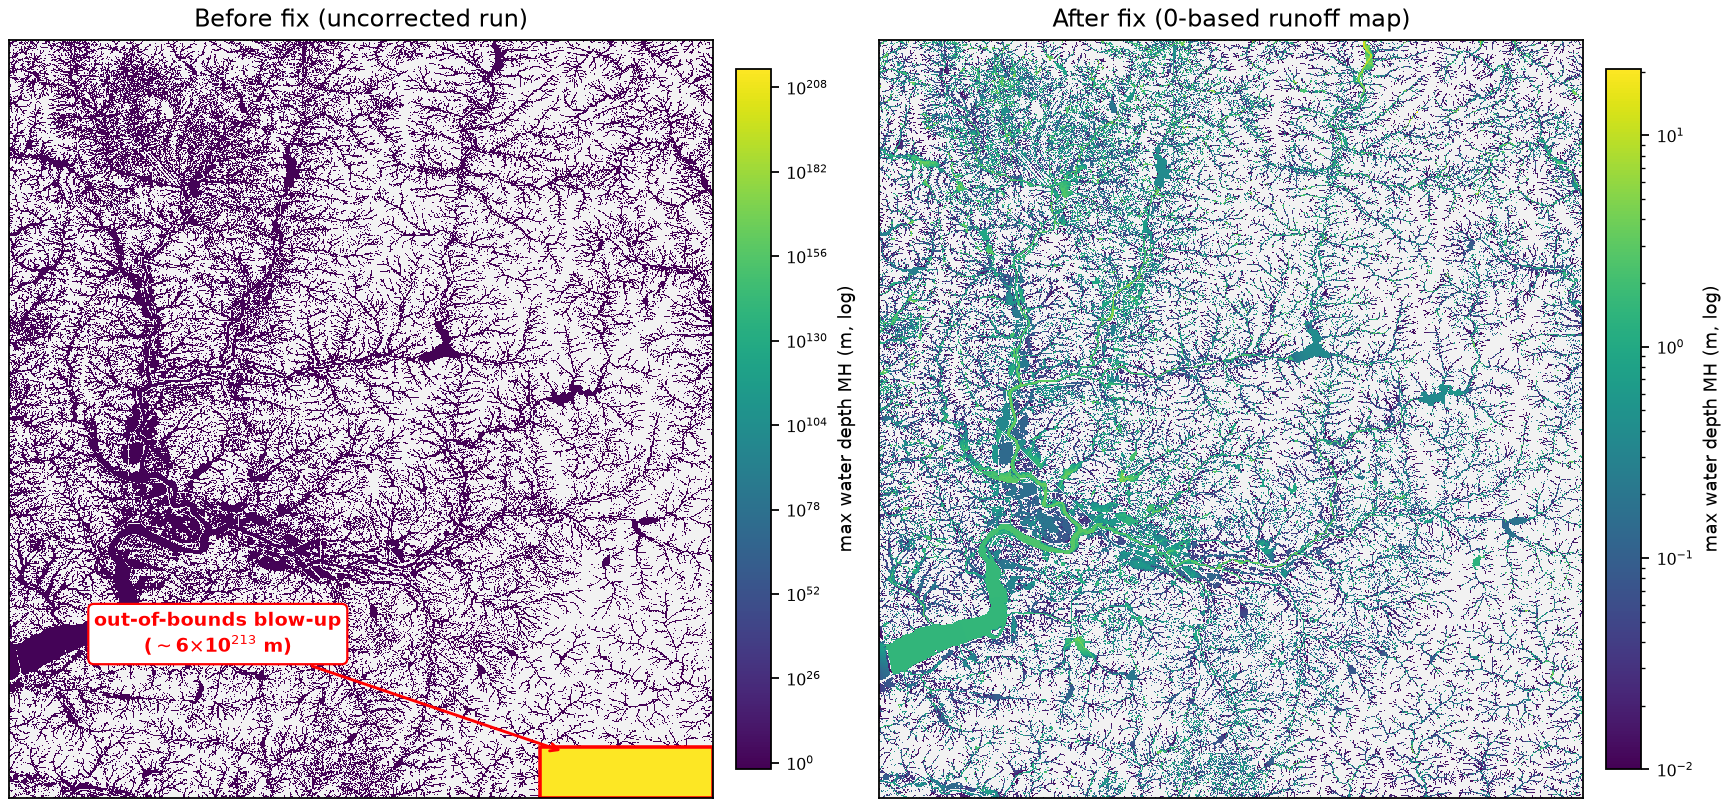
\includegraphics[width=0.60\textwidth]{figures/mh-before-after.png}
\caption{Real HPC output before and after the tool-diagnosed fix (maximum water depth,
logarithmic colour scale, dry cells left blank). \textbf{Left:} the uncorrected run---a runoff
map numbered from $1$ causes an out-of-range table read that injects a constant
$\sim$$6\times10^{213}$\,m block in the southeast (highlighted), flattening the real flood
network at the bottom of a scale spanning some $216$ orders of magnitude. \textbf{Right:} the
corrected run, numbered from $0$---realistic, terrain-following depths (maximum $20.7$\,m), and
the block is gone. Re-checking both maps with the tool reports no fault on the corrected run.}
\label{fig:beforeafter}
\end{figure*}

\section{Threats to Validity}
\label{sec:threats}

\paragraph{Can we trust the automatic judge?} The with-versus-without comparison is graded by a
language-model judge, and no such judge is perfect. The judge's \emph{design} already guards
against bias (Section~\ref{sec:scoring}): it is blind to which arm it grades, so any bias cancels
in the difference, and it grades the agent's own answer against a solver-confirmed correct
answer using a direction-appropriate set of questions. What remains is the judge's plain error
rate, which we measured directly. A domain expert re-graded \emph{all} $248$ ablation runs by
hand, without seeing the judge's verdicts---a check of the judge, not of the project labels. The
human and the judge agree $98.8\%$ of the time ($245/248$), and $100\%$ ($48/48$) on the clean
projects that carry the don't-cry-wolf claim; every re-graded run is published for
inspection~\cite{artifact-human}. All three disagreements gave a \emph{bare}-arm
answer credit that the judge had scored as a miss (in one case by leaving the run ungraded), so
the judge, if anything, slightly \emph{under}-rates the bare arm and cannot inflate the tool's
measured advantage. Two stronger, independent judges confirm that this result is not an artifact
of judge strength: re-grading every run with Opus (the primary judge's own family) and with
\texttt{gpt-5.6-sol} (a different family, which cannot share the Claude agent's self-preference)
leaves the localization advantage intact. Written as Claude/Codex points, the
\emph{+tool}-minus-\emph{bare} gap is $+18/+20$ under the primary judge, $+22/+20$ under Opus,
and $+33/+22$ under \texttt{gpt-5.6-sol}; the stronger judges agree with the primary on $95\%$
and $94\%$ of cells and rate the \emph{bare} arm no higher, so a stronger judge only widens the
gap. This concern applies only to the with-versus-without comparison: the tool's own accuracy is
checked against the real solver, not by a model (Section~\ref{sec:oracle}).

\paragraph{Could the answer key itself be wrong?} A subtler concern than judge error is that our
answer key could be wrong---an injected ``fault'' the real solver tolerates, or a ``clean''
project it rejects. The solver-as-judge pass (Section~\ref{sec:oracle}) closes one direction
outright: \emph{tool-missed}$=0$ confirms that no project the solver rejects is mislabeled clean,
and the same pass caught a genuinely mislabeled project (a rainfall file the solver in fact
rejects), on top of the test-data fix of Section~\ref{sec:fidelity}. The other direction---a
fault the solver tolerates and runs to completion---the solver cannot settle by itself; those
labels rest on the output-sanity scan and a human audit of the small residual. That the test
projects were AI-generated does not change this argument: the credibility of the labels rests on
the solver and the human audit, not on who created the files.

\paragraph{Faithfulness of the test data} As Section~\ref{sec:fidelity} shows, an input format
that does not match the real solver can quietly distort the result. We traced the solver's
source, rebuilt every binary project, and re-ran the experiment; the tool now reads the elevation
header exactly as the solver does. We checked the opposite direction too: a header the agents
kept insisting the runoff \emph{map} needed is in fact \emph{not} required (and would break the
solver), so the tool correctly treats those files as header-less. The \emph{bare} arm's remaining
misses are therefore real agent errors, not leftovers from the test data.

\paragraph{What the tool does not cover} The tool works from the setup files before a run, so
failures that appear only while the program runs---a missing software library at launch,
say---are out of scope by design; the tool complements runtime debugging rather than replacing
it. Even before a run, the tool is a fixed set of checks for \emph{known} kinds of mistakes
(Table~\ref{tab:checks}), not a general anomaly detector: a brand-new kind of fault with no
matching check will pass. Two things soften this limit. The agent still reads the files itself
and catches many faults without the tool (Section~\ref{sec:results}), so the tool's job is to
make the \emph{recurring} problems reliable, not to catch everything; and adding a check is
cheap---each is a small, self-contained function tied to one place in the solver source---so the
catalog grows as new cases appear. A self-serve way for non-programmers to add checks is left for
future work.

\paragraph{How far the results generalize} Our results cover one solver, two AI clients, and one
machine, with three repeats per faulty project and one per clean or user-rule project. We report
Wilson $95\%$ intervals for the ablation proportions (Table~\ref{tab:results})---reliable at
small samples and near $0$ or $100\%$, where the usual normal approximation is not. The
setup-fault columns ($n{=}45$) are tight enough that the localization gain
($78$--$80\%\!\to\!98\%$) clearly survives them, while the smaller Expect.\ and Clean groups
($n{=}5$, $12$) leave the false-alarm and user-rule effects directional rather than sharply
separated. The tool's own accuracy (Section~\ref{sec:oracle}) is deterministic and reproduces
exactly, so that number is a measurement rather than a sample and carries no interval. Nothing in
the architecture is TRITON-specific: the shared core, the human-in-the-loop gating, and the two
delivery surfaces carry over unchanged, and only the check catalog encodes solver-specific
invariants. Porting to another solver driven by a text configuration and input files therefore
means rewriting the checks, not the framework: an adapter mapping that solver's directives
(OpenFOAM case dictionaries, HEC-RAS parameter tables, WRF nested-domain definitions) onto the
same core, plus a solver-confirmed answer key of its own. More repeats for tighter intervals, and
that port, are left for future work.

\section{Related Work}
\label{sec:related}

\paragraph{Agentic AI for HPC and scientific workflows}
A fast-growing line of work puts LLM agents in charge of scientific campaigns on clusters:
code-first materials agents that write and run Python across several simulation codes~\cite{matclaw},
multi-agent frameworks that design experiments and launch large batches of simulations on
leadership-class machines~\cite{mada,materials-aurora}, and automated research loops that edit
training code and keep or undo each change according to a physics-based scorecard~\cite{mlipilot}.
These systems are \emph{generation- and orchestration-first}: the agent produces artifacts and drives
runs, then iterates. Closest to our aim is LARA-HPC~\cite{lara}, which argues for a
``validation-first'' approach and uses lightweight \emph{dry runs} of the simulation to catch errors
cheaply. We share that spirit but push further on safety and cost: \texttt{diagnose\_project} is
\emph{fully static}---it never runs the solver at all, not even a dry run---and the tool reads
\emph{exactly what the solver reads}, so the tool works on any hand-built TRITON project, not
only projects that a particular generation pipeline produced. Notably, MatClaw~\cite{matclaw}
reports that agents ``struggle with tacit domain knowledge''---the setup routines and file
conventions that practitioners rarely write down. Our tool encodes exactly the setup conventions
the agent would otherwise guess at, and we measure the effect that this encoding has.

\paragraph{LLM agents for code and workflow debugging}
SWE-bench~\cite{swebench} established real GitHub issues as a benchmark, and
SWE-agent~\cite{sweagent} showed that a purpose-built interface between the agent and the computer
markedly improves a model's software-engineering performance---the general version of our specific
claim that a purpose-built tool helps. Much of the follow-on work grounds its fixes in \emph{runtime}
signals: diagnoses drawn from tests that reproduce the bug~\cite{swedoctor}, and tools for inspecting
what the agent did step by step~\cite{agentstepper}. Our target is different in kind: configuration
and input faults in a scientific workflow, found \emph{statically} from the setup files before
anything runs, rather than source-code bugs found by executing tests.

\paragraph{Tool use and the Model Context Protocol}
ReAct~\cite{react} and Toolformer~\cite{toolformer} established how LLMs use tools, and MCP~\cite{mcp}
standardizes how tools are offered to agents. Several MCP servers now target HPC and quantum
execution~\cite{mcp-quantum,materials-aurora}. These servers offer \emph{execution} tools (launch
jobs, orchestrate campaigns); we contribute a \emph{read-only, static diagnosis} tool over the
same standard---and rather than only showing that the tool works, we test whether the tool
actually changes what the agent finds, through a controlled with-versus-without comparison. This
point also separates the contribution from a conventional configuration linter. Run as a
stand-alone command, the same checks would sit outside the agent's reasoning loop. Exposed over
MCP, the checks become something the agent invokes mid-diagnosis and acts on---and the $\pm$tool
comparison measures precisely that change in the agent's behavior, not merely the checks in
isolation.

To our knowledge, no prior work evaluates a \emph{static} diagnosis tool that reads exactly what the
solver reads, for a scientific solver, through a controlled with-versus-without comparison across
independent agent clients; the closest work~\cite{lara} validates inside a generation pipeline using
dry runs, and the
software-engineering line operates on code repositories by running them.

\section{Conclusion}
\label{sec:conclusion}
A small, static tool that works from a project's own setup files---and that reaches the agent
through standard interfaces---measurably improves an AI assistant's ability to catch ``works but
is wrong'' HPC faults before any compute is spent. The tool does this while \emph{reducing} the
agent's turns and cost. The result holds across two independent AI clients, and the tool's own
overhead is negligible. The compute at stake dwarfs that overhead: the operational run of
Section~\ref{sec:motivation} held $40$ A100 GPUs for some $27$~minutes---about $18$
GPU-hours---and returned a product that had to be discarded, while the static check that catches
the fault takes about a second on a laptop.

Two lessons generalize past this solver. First, test fixtures must be \emph{validated} against
the real program, not merely constructed: a missing header in our binary inputs broke no test,
yet quietly made the tool look better than it was, and we caught it only by running every fixture
through the solver. Second, these faults live exactly where a convention looks standard but is
not. The upstream pipeline numbered runoff zones from $1$, as GIS tools do, while the solver
indexes from $0$; and our tool-free agents repeatedly insisted that the runoff map needed a header
the solver in fact rejects. Both are setups that satisfy surface plausibility while violating the
solver's own semantics---which is precisely what \texttt{diagnose\_project} encodes.

\section*{Acknowledgment}
The research was supported by the US Air Force Numerical Weather Modeling
Program. The research used resources from the Oak Ridge Leadership Computing
Facility at Oak Ridge National Laboratory (ORNL), which is a DOE Office of
Science User Facility. The authors are employees of UT-Battelle, LLC, under
contract DE-AC05-00OR22725 with the US DOE. Accordingly, the publisher, by
accepting the article for publication, acknowledges that the US government
retains a nonexclusive, paid-up, irrevocable, worldwide license to publish or
reproduce the published form of this manuscript or allow others to do so, for US
Government purposes.

\bibliographystyle{IEEEtran}
\bibliography{references}


% The AD/AE appendix follows the references, per SC convention, and starts on its own
% page: pages 1--10 are then the paper and its bibliography with nothing else on them,
% so the appendix is separable at a glance if the 10-page limit excludes it.
\clearpage
\appendices
\section{Artifact Description / Artifact Evaluation}
\label{sec:reproducibility}

\subsection*{Artifact check-list}
\emph{Program:} \texttt{diagnose\_project}, a static setup-file checker for the TRITON flood
solver, delivered as an MCP server and a VS~Code language-model tool.
\emph{Build:} TypeScript via \texttt{npm ci}; the solver from TRITON upstream commit
\texttt{267ebc25f} (clean tree) with CMake~3.28 and \texttt{mpic++}~13.3 (GCC), Kokkos
\emph{Serial} backend, CUDA disabled---the recorded environment ships with the bundle.
\emph{Data set:} 32 TRITON projects (20 faulted, 12 clean), 828\,KB, plus the graded run
records and the four reviewer artifact pages, which carry the answer, gold label, and
verdict for every one of the 248 ablation runs.
\emph{Run-time environment:} Ubuntu~24.04.4 LTS (kernel~7.0.0), Node~22.22.2,
Python~3.12.3, \texttt{jq}~1.7, bubblewrap~0.9.0; no root access needed.
\emph{Hardware:} Layers~1--2 need only a commodity x86-64 machine---ours was a 4-core Intel
Core~i5-4250U with 7\,GB RAM. The operational run of Figures~\ref{fig:anomaly}
and~\ref{fig:beforeafter} used 40 NVIDIA~A100 GPUs (10 nodes $\times$ 4) on a private
cluster at the Oak Ridge Leadership Computing Facility.
\emph{AI clients:} Claude Code~2.1.221 (\texttt{claude-sonnet-5}) and Codex CLI~0.144.5
(\texttt{gpt-5.6-sol}); blind judge \texttt{claude-sonnet-5}.
\emph{Metrics:} those of Tables~\ref{tab:results} and~\ref{tab:efficiency}, one layer each.
\emph{Disk and time:} the bundle is 2.8\,MB compressed (191 files) and is built from the
repository's tracked content alone, so it rebuilds byte-for-byte from a fresh clone;
Layer~1 finishes in seconds, Layer~2 is 32 short single-core solver runs, and Layer~3 is
248 agent runs and the only layer that costs money.
\emph{Availability:} \url{https://github.com/grnydawn/triforge-extension-agenticai4hpc} plus an
archived deposit\todo{Zenodo DOI once reserved}; code under MIT, data under
CC~BY~4.0.

\paragraph{Layer~1 --- fully automatic, no AI needed} The tool-level result of
Section~\ref{sec:results} reproduces with no access to any AI service. \texttt{npm ci} installs the
pinned dependencies; \texttt{npm run test:unit} runs the unit tests (the pure diagnosis core, the
file-access helpers, and the test-set scorer); and \texttt{npx tsx scripts/eval/diagnose-report.ts}
re-runs all \textbf{32} projects under \texttt{eval/diagnose-corpus/} against their answer key and
rewrites \texttt{report.json}. The run prints \emph{detection~$100\%$ $\cdot$ isolation~$100\%$
$\cdot$ clean~precision~$100\%$}; comparing the regenerated \texttt{report.json} against the
committed copy confirms the numbers exactly. The regenerated report is also published as a
browsable online artifact~\cite{artifact-tool}.

\paragraph{Layer~2 --- checked against the real solver, still no AI} The claim that the answer key
itself is correct (Section~\ref{sec:oracle}) reproduces with the TRITON build under
\texttt{eval/diagnose-corpus/build} but \emph{no} AI service.
\texttt{scripts/eval/run-triton-oracle-corpus.sh} runs every project through the real solver and
records what it did (reject at startup~/ run to completion~/ run then crash) to
\texttt{oracle-report.json}; \texttt{three-tier-corpus.sh} then adds an automatic output-sanity scan
(\texttt{output-sanity.ts}, itself covered by unit tests in \texttt{test/unit/eval/}) and reconciles
each project's label against the answer key, checking that no \texttt{clean} project is in fact
rejected by the solver; \texttt{build-verdict.ts} produces the per-project reviewer dataset. This is
the reproducible evidence that \emph{tool-missed}$=0$ and that every label agrees with the solver;
the resulting dataset is the online artifact of Section~\ref{sec:oracle}~\cite{artifact-oracle}.

\paragraph{Layer~3 --- the with-versus-without comparison} The two-arm result needs both AI
clients and network access to their services, so it is not self-contained.
\texttt{scripts/eval/run-study.sh} drives each client for every project and arm inside the sandbox of
Section~\ref{sec:method} (a hidden home directory with only the toolchain exposed);
\texttt{judge-results.sh} grades each saved transcript with the blind judge, which also writes a
one-line reason per run, and \texttt{mcp-overhead.py} measures the tool's communication cost. The
inputs are the 32 projects and the two instructions (\emph{+tool} with the tool, \emph{bare}
without). The graded transcripts, metrics, and overhead measurements are published as a browsable
online artifact~\cite{artifact-ablation}.

\paragraph{Layer~4 --- the judge itself, audited} The agreement figures of
Section~\ref{sec:threats} validate the \emph{grader} rather than reproduce the result, so they
form a fourth layer. A domain expert re-graded all \textbf{248} ablation cells by hand without
seeing the judge's verdicts; \texttt{runs/human-judge-evaluation.csv} records for each cell the
client, arm, fixture, trial, gold label, judge verdict, human verdict, and a one-line note, and
tallies the $245/248$ agreement quoted in Section~\ref{sec:threats}. Two further sheets,
\texttt{clean-cell-human-audit.csv} and its phase-2 companion ($32$ and $48$ rows), audit the
clean-project cells that carry the don't-cry-wolf claim. The human pass is a record rather than a
script, so re-running it means re-grading: the browsable artifact~\cite{artifact-human} presents
all 248 answers with their gold labels for exactly that. The multi-judge check \emph{is}
re-runnable---\texttt{scripts/eval/judge-multi.sh} re-grades the same 248 saved answers under Opus
and \texttt{gpt-5.6-sol}; \texttt{runs/robustness/README.md} carries the resulting per-judge
tables, and the per-cell verdicts regenerate beneath it.

\end{document}
